\documentclass[10pt,a4paper]{article}
\usepackage{amsmath}
\usepackage{float}
\usepackage{graphicx}
\title{Advanced Computer Architecures notes}
\author{Elia Ravella}
\begin{document}
	\begin{titlepage}
		\maketitle
	\end{titlepage}
	
	\tableofcontents
	\clearpage
	
	\part{Introduction}
		\section{Taxonomy of Computer Architectures}
			\subsection{Flynn Taxonomy}
				Flynn defined four categories to group computing architectures. This so called taxonomy helps system architects to distinguish among possible models of processors or system themselves. 
				\begin{enumerate}
					\item SISD: Single Instruction Single Data, uniprocessor systems;
					\item MISD: Multiple Instructions Single Data, no commercial application;
					\item SIMD: Single Instruction Multiple Data, low overhead, used in custom integrated circuits;
					\item MIMD: Multiple Instruction Multiple Data, off the shelf micros
				\end{enumerate}
				SISD is the simplest and most diffuse model of computation, one data stream in input and a \emph{single} instruction executed per istant of time. SIMD introduces parallelism in a vector fashion: multiple processes execute a single instruction (the \emph{same} instruction) on different data elements. Another type of parallelism: MIMD. Just SIMD with multiple different instructions per instant.\\
				
	\part{Performance and Cost}
		\section{Performance}
			\subsection{Evaluating performance}
				We need to distinguish between how to measure performance of a computer architecture and what impacts it without affecting performance. The amount of memory used is not a performance evaluator, but it affects performance in some way. The power consumed, the latency and the execution time are. To evaluate the performance of a CA I must use all the performance indicator and find the right tradeoff. Also, context! A CA is inserted in a context that bounds its scope, so the environment itself shapes the way performance is evaluated\\
				\emph{Every performance indicator} says something about the CA. So, the whole system must be evaluated with a \emph{whole set} of indexes that each tell a different thing about the system itself. This provides a full view of the system strenghts and weaknesses and highlights the things to optimize.
				
			\subsection{Quantifying the Design Process}
				"The frequent case" case: when designing a CA, the "frequent case" represents the set of conditions met \emph{the most times} during a standard computation run. Optimizing the standard case means optimizing \emph{singnificately} all the system behaviour. 
				
				\paragraph{Amdahl's Law}
					Amdahl's law describes the concept of the speedup as a function of execution time. The set of formulas that describes the law is
					\begin{equation}
						EXTIME_{new} = EXTIME_{old} \times [(1-Fraction_{enhanced}) + \frac{Fraction_{enhanced}}{Speedup_{enhanced}}]
					\end{equation}
					\begin{equation}
						SPEEDUP_{overall} = \frac{EXTIME_{old}}{EXTIME_{new}} = (1-Fraction_{enhanced} + \frac{Fraction_{enhanced}}{Speedup_{enhanced}})^{-1}
					\end{equation}
					and calculates the speedup of a system taking into account all his part, the speedupped one and the invariate one.\\
			
			\subsection{Indexes on performance}
				Overview of performance indicators and measurements.
				\begin{itemize}
					\item Instruction Count: the effective number of instructions executed. This is influenced also by the program we're trying to execute.
					\item Tyme per Cycle: the clock rate. OBVIOUSLY influenced by the hardware architecture.
					\item MIPS and MFLOPS indicates already a very \emph{program bound}-like perfomance indicator. They represents the number of integer/floating point operations that the architecture can carry out in a second. They're very synthetic indexes.
					\item CPI - Average CPI (clock per instruction) represents obviously yhe amount of clock cicles that are necessary to carry out a specific operation. The element that most impacts the CPI is the ISA: the alphabet we use shapes the words we can create. 
				\end{itemize}
				Notice how execution time is not present. That's because \emph{reducing execution time is the goal}, so execution time does not modify performance, it just \emph{represents} it. 
			
			\subsection{Benchmarking}
				Benchmarking is "running a fake program with the sole purpose to evaluate a system and find bottlenecks". It's a technical test. Workloading a CA means feeding it with a real work load to test what is a response to a non-syntethic stimulus.\\
				Benchmarking must be
				\begin{enumerate}
					\item representative: we need to benchmark the right aspects of the architecture we're testing.
					\item updated: old benchmark does not test the architecture well, because of the very architecture is changed and the benchmark is \emph{not anymore representative} because it's \emph{old}.
				\end{enumerate}
			
			\subsection{Energy, Power}
				Energy and power consumption are a "cost - like" performance indicator. The less the power, the less the cost of keep the architecture running, and tha's easy. Also, reducing the power consumed means \emph{reducing the power needed from a battery} and this impacts a lot in the mobile scenario. Energy per task is a good indicator for energy consumption. The power used by an architecture is influenced by a ton of factors, not least the TDP (thermal design power). Also architecture-bound aspects (clock rate, voltages, busses) influence power consumption \emph{heavily}.

	\part{Pipelining}
		\section{MIPS architecture}
			Reference architecture for this course is MIPS.\\
			MIPS is a RISC architecture (Reduced Instruction Set Computer) this means that the only possible operation (that are very optimized) are basic operations. This kind of architecture is the opposite of CISC (Complex ISC) where more complex operation are supported at chip level.\\
			MIPS is a LOAD/STORE architecture. This means that data cannot come into the ALU from anywhere besides the CPU general purpose registers. MIPS uses 32-bit instructions that can be
			\begin{itemize}
				\item Register Register operations
				\item Register Immediate operations
				\item Branch operations
				\item Jump/Call operations
			\end{itemize}
			Operand lenght is 6-bit. We have 64 possible operations.\\
			
			\subsection{Assembly basics}
				We'll see three classes of MIPS instructions:
				\begin{itemize}
					\item ALU: add "reg target" "reg source" "reg source", or sub "reg target" "reg source" "immediate"
					\item LOAD/STORE: lw "reg target" "offset register" (load word)
					\item Branches/Jumps: classic bne or bge or jmp operations
				\end{itemize}
			
			\subsection{MIPS instruction execution}
				A fetch - decode - execute cycle in this architecture works this way:
				\begin{enumerate}
					\item Fetching the instruction means sending the PC content to the memory in order to access the memory location where the instruction is. Then, the PC is updated (PC + 4, each instruction take 32 bits).
					\item Decoding the instruction: in this phase a fixed-field operation is put in place to deconde the instruction itself, and the registers needed for the computation are read.
					\item Execute operation: the ALU calculates the result of the instruction supplied.
					\item Memory Access and Write Back phases: in these two phases the CPU takes care of the memory access (LOAD or STORE instructions) and the registers update.
				\end{enumerate}

				
			\subsection{MIPS Chip Architecture}
				\begin{figure}[H]
					\centering
					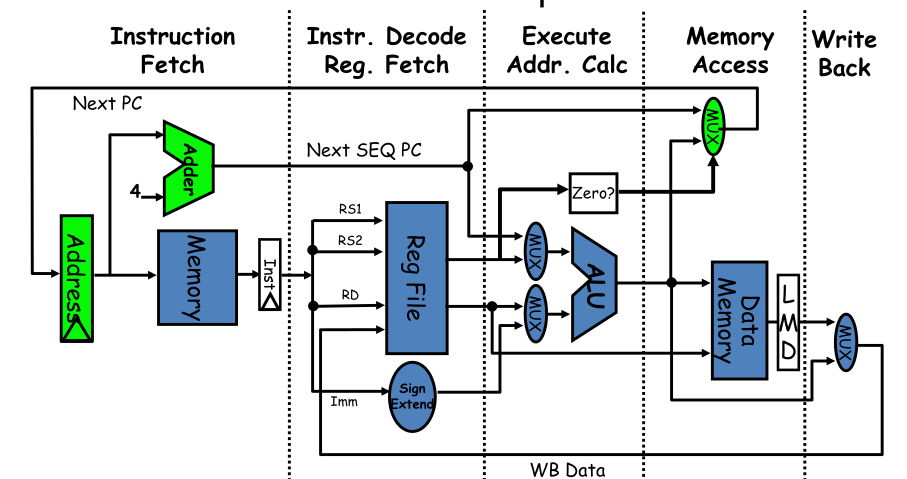
\includegraphics[width = \textwidth]{./images/MIPSDP.png}
					\caption{The MIPS data path with pipeline stages highlighted}
				\end{figure}
				
				\begin{figure}[H]
					\centering
					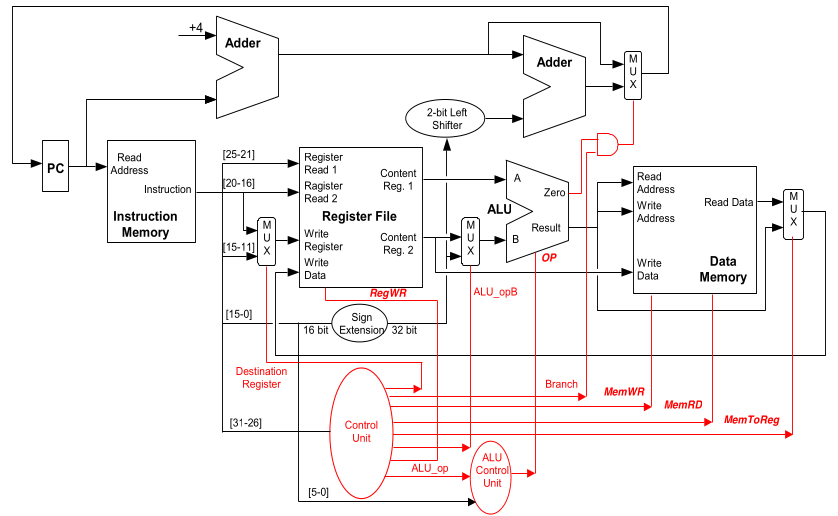
\includegraphics[width = \textwidth]{./images/MIPSCPU.png}
					\caption{The MIPS full CPU, data path integrated with control unit}
				\end{figure}
				
				\begin{figure}[H]
					\centering
					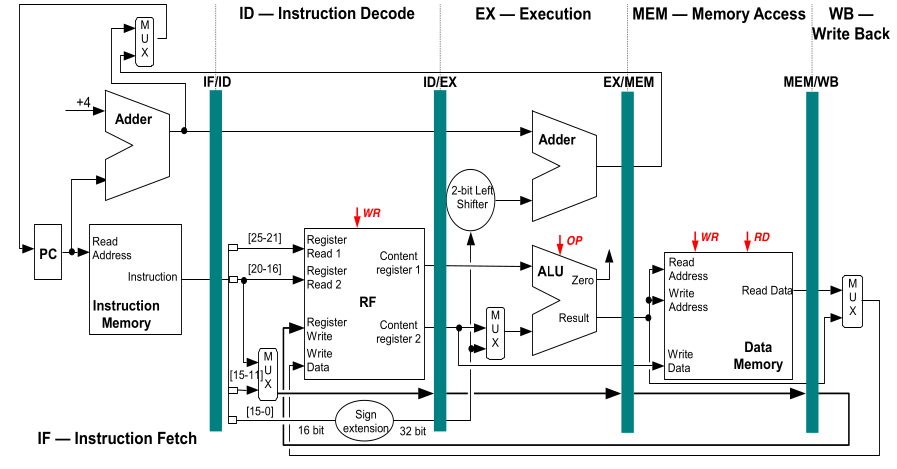
\includegraphics[width = \textwidth]{./images/MIPSCPUPIPELINED.png}
					\caption{Pipelined MIPS}
				\end{figure}
				
				
		\section{Data and Control}
			Every computer architecture is composed of 2 main parts: the one that computes data (datapath) and the one that controls the execution (control unit).
			
			\paragraph{Datapath}
				The datapath runs the house. All data pass through this module, and the registers here are used to pipeline operation.
			
			\paragraph{Control Unit}
				The CU guides the computations. It takes "run time decisions" in order to pilot execution of intructions. The registers here are architecture-specific.
				
			\paragraph{Memory}
				And memory? "Slow primary memory" is connected with the CPU (so DP + CU) by means of buses. The structure is similar to:
				\begin{figure}[H]
					\centering
					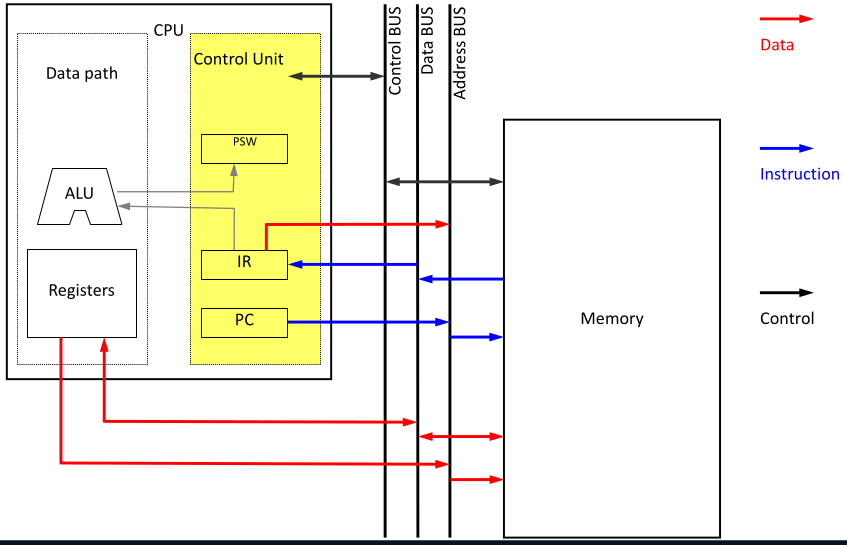
\includegraphics[width = \textwidth]{./images/ArchBuses.png}
				\end{figure}
				Things to be noted:
				\begin{enumerate}
					\item the datapath does not connect to the control path
					\item the control unit does not write on the data bus
				\end{enumerate}
			
\end{document}



















